\section{Cluster Structures}

From the experimental results we can obtain two hints for the cluster
structure: the minimum size and the xenon content. We will in the following
use these to construct possible cluster structures for which we will later
simulate the ICD and ETMD spectra. At this step we put in whatever structure
we might think of and hope to be able to exclude some of them by comparison of
the ICD and ETMD spectra to the experimental electron-electron coincidence
spectra.

The expected mean argon cluster sizes
were estimated and collected in Table \ref{table:cluster}.
In case of the smaller clusters measured
these expectation values range from \unit[3 -- 21]{Ar atoms} for
expansion of pure argon. The cluster sizes of a mixed gas are unknown but
for xenon as the second component the cluster sizes can be expected to
be larger than those of pure argon due to the higher polarizability
and hence larger cohesive energy of xenon. All clusters
contributing to the coincidence spectrum
do contain at least one xenon atom, otherwise there would be no signal at all.
In an expansion a large variance of clusters and with different structures
is produced. However, for small clusters consisting of less than
approximately \unit[1000]{atoms} so-called \emph{islands of stability} were
found for clusters with icosahedral shape. This means, that the probability
to find and measure such a cluster is higher than a different structure.
We therefore started from icosahedral structures and substituted atoms
in the clusters by
argon / xenon atoms or added these to a given structure close to the wanted
position. Afterwards the cluster structures were optimized using the
UFF force field \cite{} implemented in
Avogadro \cite{} for a structure optimization.

\begin{figure}[h]
 \centering
 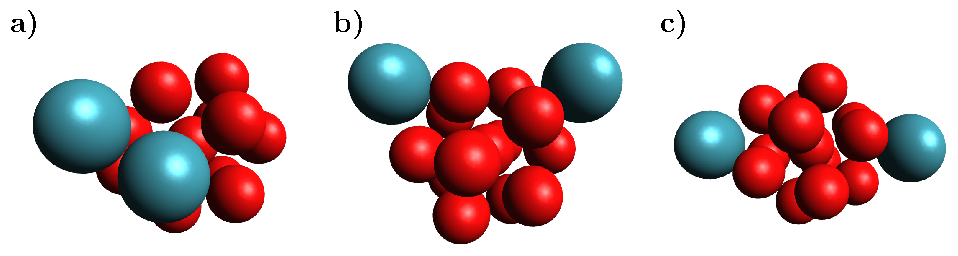
\includegraphics[width=8.5cm]{pics/cluster_2_overview.pdf}
 \caption{Cluster structures with 13 argon atoms and two additional xenon
          atoms on different surfaces of the argon icosahedron:
          \textbf{a)} closest possible \textbf{b)} middle \textbf{c)}
          furthest away.}
 \label{figure:cluster_2_overview}
\end{figure}

\begin{figure}[h]
 \centering
 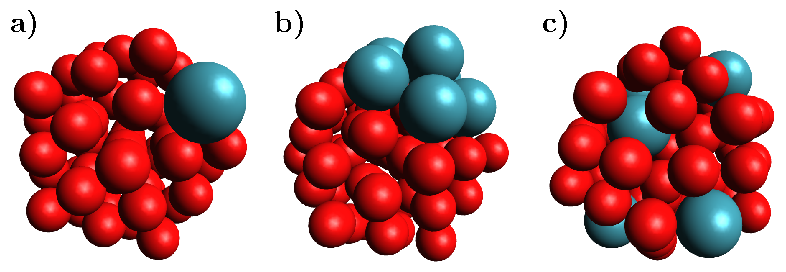
\includegraphics[width=8.5cm]{pics/cluster_3_overview.pdf}
 \caption{Cluster structures based on 55 atoms icosahedral cluster structure.
          \textbf{a)} 1 xenon atom on the surface of a 55 atoms icosahedral
          argon cluster. \textbf{b)} six xenon atoms inside a 55 atoms cluster
          grouped on one side. \textbf{c)} six xenon atoms distributed
          in a 55 atoms cluster. }
 \label{figure:cluster_3_overview}
\end{figure}

As discussed in the introduction, the small clusters are very likely
to deviate from a core-shell structure with a xenon core surrounded
by argon shells as observed for large clusters. We therefore start from
argon clusters of 13 or 55 atoms and modify them in one of the following
ways:

\begin{itemize}
 \item add one xenon atom on top of a surface / edge / vertex of
       the argon core as for example shown in
       Figure \ref{figure:cluster_3_overview} Panel a)
       for one additional xenon atom
       on top of surface of a \unit[55]{atoms} argon core
 \item substitute one argon atom in a surface / edge / vertex position if
       possible
 \item substitute one or two argon atoms in the core of the argon cluster
       by xenon atom(s) for the simulation of the core-shell structure
 \item add two xenon atoms on top of surfaces of a 13 atoms argon core
       in different relative positions (see Figure
       \ref{figure:cluster_2_overview})
       in order to achieve a xenon content in the cluster close to the
       measured one shown in Table \ref{table:cluster}
 \item substitute six argon atoms of a 55 atoms argon cluster by xenon
       atoms either grouping them or scattering them througout the cluster
       (see Figure \ref{figure:cluster_3_overview} Panels b) and c)) in order to
       achieve a xenon content in the cluster close to the experimental one
\end{itemize}

Furthermore we constructed a core-shell structure with a core of
1415 xenon atoms and one additional complete layer of argon atoms for
comparison with the largest measured ArXe clusters.


